\section{数据探索与预处理}

\subsection{数据概况}

原始数据集共 50,000 条记录，包含 23 个字段。其中 4 个分类变量（education\_level、city\_type、current\_vehicle\_type、ev\_adoption\_likelihood）、2 个二值变量（home\_charging\_available、previous\_ev\_experience）、14 个连续数值变量，以及 3 个目标变量（monthly\_energy\_consumption\_kwh、monthly\_charging\_cost、fuel\_expense\_per\_month）。

数据质量总体良好：无重复行、无无穷值、无常量列。存在三处缺失：education\_level、charging\_station\_accessibility、ev\_knowledge\_score 各缺失 500 条（各占 1\%），缺失模式近似随机。另有两处值得注意的分布特征：fuel\_expense\_per\_month 存在 271 个负值（最小值 $-99.7$），属业务语义上的异常；electricity\_cost\_per\_kwh 范围为 0.08--0.35，共 28 个离散取值。

三个任务的目标变量分布如表\ref{tab:target_dist}所示。

\begin{table}[H]
\centering
\caption{目标变量分布}
\label{tab:target_dist}
\begin{tabular}{ccccc}
\toprule
\textbf{任务} & \textbf{目标} & \textbf{均值 $\pm$ 标准差} & \textbf{范围} & \textbf{偏度} \\
\midrule
任务一 & 月能耗 & $186.74 \pm 88.25$ & 15.6--645.9 & 0.539 \\
任务二 & 充电成本 & $40.24 \pm 24.94$ & 1.4--199.6 & 1.067 \\
任务三 & 燃油支出 & $295.17 \pm 130.18$ & $-99.7$--862.0 & 0.104 \\
\bottomrule
\end{tabular}
\end{table}

\subsection{数据生成机制识别}

在进入建模之前，本文首先通过比率诊断与相关分析，识别数据背后近似确定性的生成机制。这一``先结构、后模型''的思路贯穿全文。

\subsubsection{核心相关性}

如图\ref{fig:corr}所示，三个目标与对应的出行变量之间存在极强的线性关系：月能耗与周里程的 Pearson 相关系数为 0.936，燃油支出与日通勤里程的相关系数为 0.952，充电成本同时受月能耗（0.765）与电价（0.584）驱动。这一相关性结构为后续的稀疏建模提供了直接依据。

\begin{figure}[H]
\centering
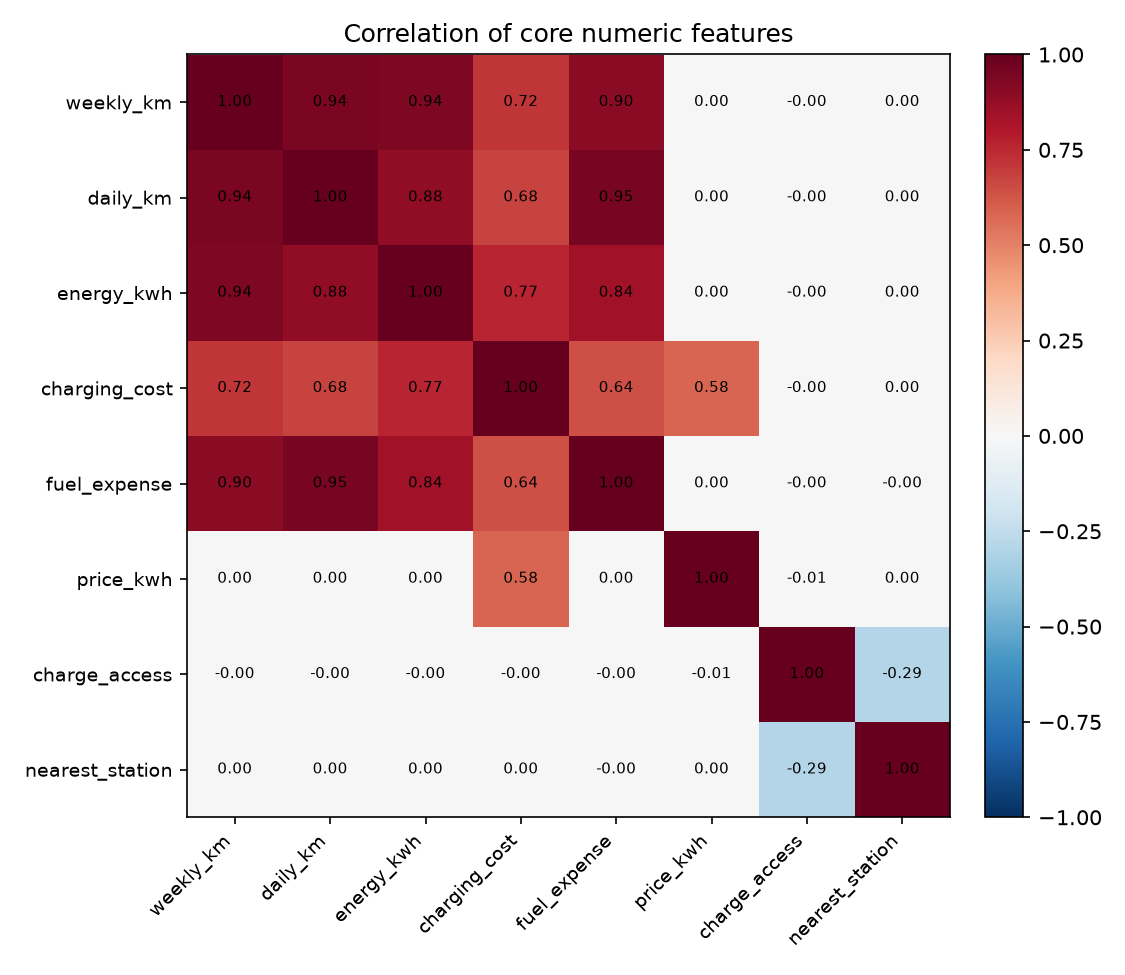
\includegraphics[width=0.85\textwidth]{figures/correlation_heatmap.png}
\caption{核心数值特征相关性热力图}
\label{fig:corr}
\end{figure}

\subsubsection{比率诊断}

进一步，本文考察若干关键比率变量的分布，以验证其是否服从某种随机生成机制：

\begin{enumerate}[itemsep=0pt]
\item \textbf{周里程/日通勤}：均值 6.50、标准差 0.87，与均匀分布 $U(5,8)$ 的理论均值（6.5）与标准差（0.866）高度吻合，表明周里程约为日通勤的 5--8 倍随机倍数；
\item \textbf{月能耗/周里程}：均值 0.816、范围 0.60--1.03，近似一个与其余特征无关的随机量，说明周里程是能耗的核心驱动变量；
\item \textbf{燃油支出/日通勤}：拟合过原点 OLS 得系数 8.395，残差标准差约 40，与公式 $fuel \approx 8.4 \times daily + N(0,40^2)$ 一致；
\item \textbf{充电成本/(能耗 $\times$ 电价)}：以能耗与电价的乘积预测成本，得到 $R^2=0.9994$，说明充电成本几乎由该乘积完全确定。
\end{enumerate}

上述机制意味着：题面提示的车型交互、地域差异等复杂映射在当前数据中并不存在，简单模型反而更贴近真实的数据结构。

\subsection{数据清洗流水线}

完整预处理流程由单一 Python 脚本实现，全链路可复现。步骤如下：

\begin{enumerate}[itemsep=0pt]
\item \textbf{Schema 校验}：每次训练前自动检查文件 SHA-256、行数、列名与顺序、类型、目标存在性、重复行、缺失、无穷值、非法类别与数值边界，结果写入 JSON 报告；
\item \textbf{固定折划分}：以随机种子 42/2026/7 生成 3 组 5 折划分，三任务共用同一组 fold\_id，保证跨任务可比与可复现；
\item \textbf{分类缺失值填充}：education\_level 的 500 个缺失位置以字符串``Missing''填充，作为独立类别参与建模；
\item \textbf{数值缺失值填补}：charging\_station\_accessibility 与 ev\_knowledge\_score 以训练折中位数填补（折内拟合，验证折只应用）；
\item \textbf{异常值处理}：fuel\_expense\_per\_month 的 271 个负值予以保留，不做截断或对数变换——这一决策由消融实验支撑（详见任务三）；
\item \textbf{编码}：线性模型对分类变量做 One-Hot（drop first），数值列标准化；树模型保留类别 dtype 与原生缺失处理。
\end{enumerate}

\subsection{最终数据规格}

清洗后数据保持 50,000 行，特征矩阵在 One-Hot 编码后为 27 维（14 个标准化数值列 + 11 个 One-Hot 列 + 2 个二值列）。三项任务的建模均以该流水线为统一入口，所有填补与编码均在交叉验证的折内完成，杜绝信息泄漏。
